

\section{Background and Challenges}
\label{subsec:preliminaries}

We aim to learn a generation model
$p_{\theta} (\y) = \prod_{t=0}^T p_{\theta}(y_t | \y_{<t})$, where
$y_t$ is a token from a vocabulary $\mathcal{V}$. The distribution at each step $t$ is obtained by applying softmax on the logits $f_\theta(y | \y_{<t})$:
\begin{equation}
\small
\begin{split}
    p_\theta(y_t | \y_{<t}) = \frac{\exp f_\theta(y_t | \y_{<t}) }{ \sum_{y'\in\mathcal{V}} \exp f_\theta(y' | \y_{<t} ) }.
\end{split}
\label{eq:softmax-logit}
\end{equation}
Despite its popularity, MLE-based training only applies when clean supervised data $\bm{y}^*$ is available, and cannot be used to optimize arbitrary task metrics (e.g., BLEU, entailment score) which are typically the goal in many text generation tasks. 
\label{sec:background:rl}
Previous research has formulated text generation as an RL problem by considering the following finite-time Markov Decision Process (MDP). 
At each time step $t$, let the ``state'' be $\bm{s}_t = \bm{y}_{< t}$, namely the partial sequence generated so far. The model (``agent'') takes as input the current state $\bm{s}_t$ and outputs a token (``action'') $a_t \in \mathcal{V}$ according to a policy $\pi(a_t | \bm{s}_t)$. 
The agent then receives a reward $r_t = r(\bm{s}_t, a_t)$ and deterministically transitions to next state $\bm{s}_{t+1}$ (i.e., the concatenation of the tokens in $\s_t$ and the new token $a_t$). 

Following the notation convention in RL, let $\tau$ be the trajectory (i.e., text sample) generated by the policy. The agent's objective is to maximize the accumulative reward,
$J(\pi) = \mathbb{E}_{\tau \sim \pi}\left[ \sum^T_{t=0} \gamma^t r_t \right]$,
where $\gamma$ is the discount factor.
A central concept in RL is the $Q$-function of policy $\pi$, $Q^\pi(\s_t, a_t)=\E_{\pi}\left[ \sum_{t'=t}^T \gamma^{t'} r_{t'} \mid \s_t, a_t \right]$, the expected future reward of taking action $a_t$ (i.e., generating token $a_t$) in state $\s_t$ and continuing with the policy $\pi$. 

\noindent\textbf{Challenges. } Text generation poses significant challenges to RL, particularly because (1) the reward signal is usually sparse, i.e., $r_t = 0,\ \forall t<T$ and the agent receives a non-zero reward $r_{T}$ only after it generates the full sequence, (2) the action space (i.e., the vocabulary $\mathcal{V}$) is extremely large.
The challenges have led to difficulties of the two major families of RL approaches applied to text generation problems, as detailed below.

\noindent\textbf{Policy-based RL}
techniques directly parameterize the policy $\pi_{\theta}$ with parameters $\btheta$. Thus the policy $\pi_{\theta}(a_t | \s_t)$ exactly corresponds to the above generation model $p_{\theta}(y_t | \y_{<t})$. 
\emph{Policy gradient (PG)} is one of the most widely used algorithms for text generation \citep{ranzato2015sequence}.
It optimizes the cumulative reward with the policy gradient using the estimated $Q^{\pi_\theta}$ value based on sample $\tau$. PG is an \textit{on-policy} algorithm, meaning that the sample $\tau$ needs to come from the the current policy $\pi_\theta$ itself.
In practice, however, optimizing this objective alone from scratch is unlikely going to work because most samples $\tau\sim\pi_\theta$ are just gibberish with zero reward, failing to provide meaningful training signals for updating the policy. 
Previous literature either initializes the policy $\pi_{{\theta}}$ with MLE training, and/or use a combination of MLE and PG updates, which often leads to marginal gains in practice~\citep{wu2018study,Choshen2020On}. 



\noindent\textbf{Value-based RL}
techniques, such as \emph{$Q$-learning}, implicitly learn the policy $\pi$ by approximating the value $Q^{\pi}(\bm{s}, a)$ directly.
Deep $Q$-learning~\citep{mnih2013playing} parameterizes the $Q$-function as $Q_\theta(\x,a)$, and train the parameters by minimizing the following regression objective $\loss(\btheta)$ based on the Bellman temporal consistency:
\begin{equation}
\small
    {\E}_{\pi'}\left[ \frac{1}{2} \left( r_t {+} \gamma \max_{a_{t+1}} Q_{\bar{\theta}}(\s_{t+1}, a_{t+1}) {-} Q_{\theta}(\s_t, a_t) \right)^2 \right]%
\label{eq:q-regression}
\end{equation}
where $\bar{\btheta}$ is the parameters of the \emph{target} $Q$-network, which is a slow copy of $\btheta$ and considered as constant for gradient computation of $\btheta$. 
Here $\pi'$ is an \emph{behavior policy} which can be an arbitrary distribution over text, such as the data distribution or replay buffer \citep{mnih2013playing}. 
This makes $Q$-learning an \textit{off-policy} algorithm because of its ability to use samples coming from other policies. After learning $Q_\theta$, one can induce a policy $\pi$ from it that takes $\arg\max_{a} Q_\theta(\s, a)$ at each state $\s$.
\citet{jaques2017sequence} instead sample tokens from the softmax function applied to $Q_\theta$.

However, the training can be unstable and inefficient due to several challenges: 
{\bf (1)} The bootstrapping nature of the above regression problem can make the training unstable. That is, the regression target $r_t + \gamma \max_{a_{t+1}} Q_{\bar{\theta}}(\s_{t+1}, a_{t+1})$ itself is derived from the $Q$-function to be learned \citep{kumar2019stabilizing}. The problem is exacerbated in the presence of sparse reward in text generation, where the real observed signal $r_t$ is zero for all intermediate $t<T$; 
{\bf (2)} The large action space (e.g., $10^4$) in text generation results in slow updates. In particular, notice that Eq.\eqref{eq:q-regression} applies the gradient update to the $Q_{{\theta}}$-value of the \emph{only one} particular token $a_t$ (out of, say, the $10^4$ candidate tokens in the vocabulary), making the training inefficient;
{\bf (3)} Besides, pure off-policy updates could be highly sensitive to the quality of training data, and miss the opportunity of on-policy exploration that maximizes the reward of interest in a more direct way.



\begin{figure*}
    \centering
    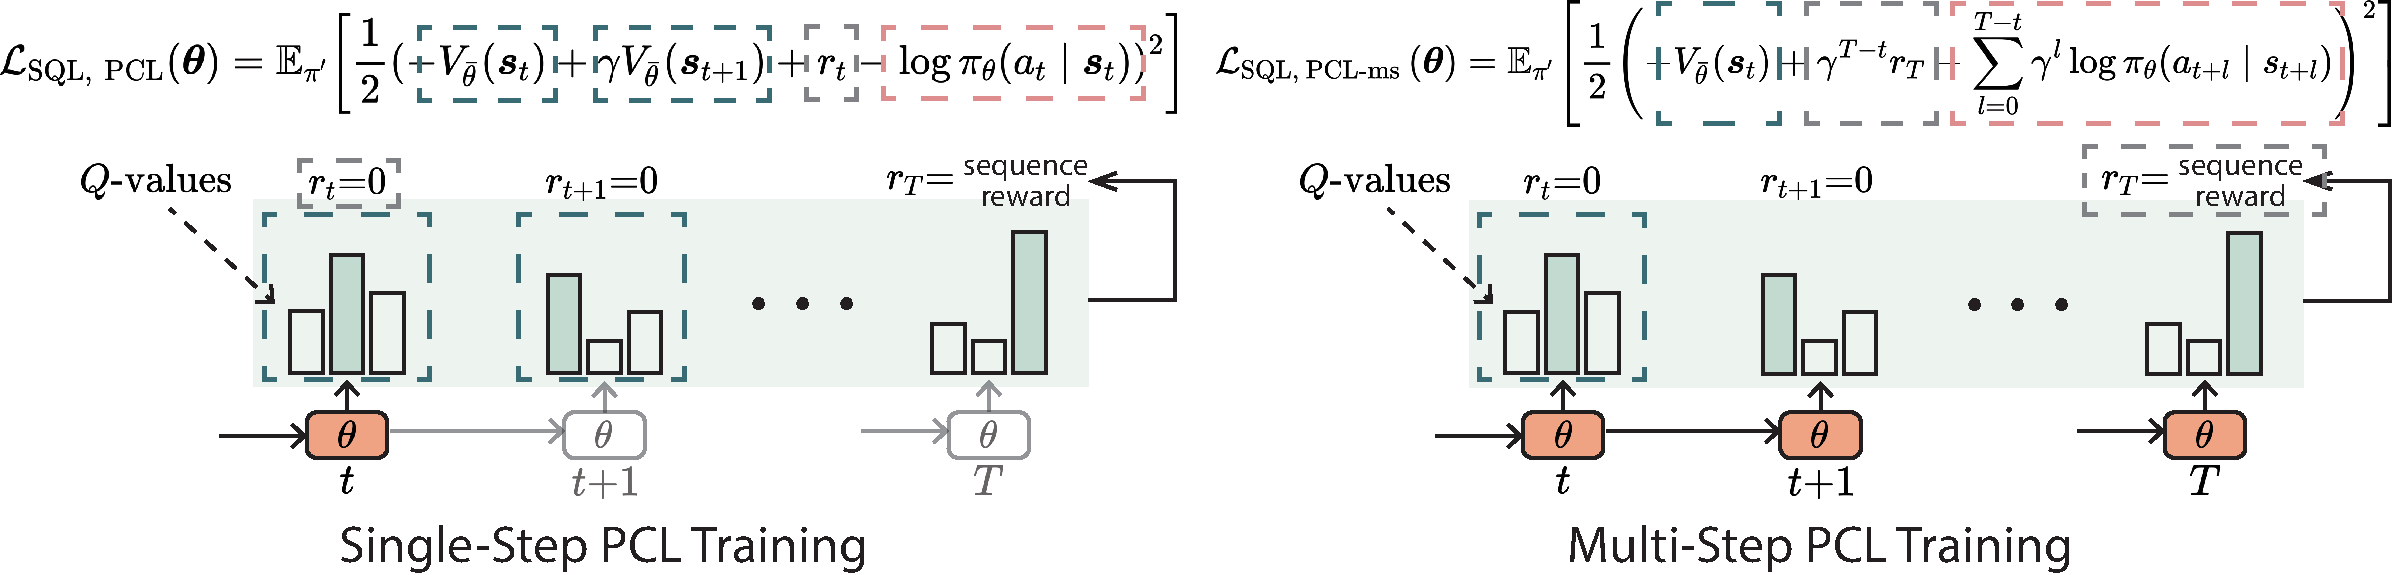
\includegraphics[width=0.99\linewidth]{figures/soft-q-learning.pdf}
    \vspace{-4pt}
    \caption{
    Soft $Q$-Learning with path consistency learning (PCL) objectives.
    {\bf Left:} Single-step objective (Eq.\ref{eq:pcl-loss}), where for each $(\s_t, a_t)$, the computation involves step $t$ and $t+1$. Dashed boxes in \textcolor[HTML]{3A6B73}{\textbf{dark green}} and \textcolor[HTML]{808285}{\textbf{gray}} indicate the regression target, where the intermediate reward $r_t$ is often 0 due to sparsity. The gradient is applied to parameters $\btheta$ at step $t$ (indicated by {\textcolor{orange}{\textbf{orange}}} color). {\bf Right:} Multi-step objective (Eq.\ref{eq:multi-loss}) which aggregates from step $t$ all the way to $T$. In this way, the final-step non-zero reward $r_T$ is used as the regression target.
    }
    \vspace{-4pt}
    \label{fig:soft-q-learning-pcl}
\end{figure*}



\section{The Soft $Q$-Learning Framework}


We introduce the soft $Q$-learning (SQL) formulation of text generation. It is seamlessly compatible with the common architecture of text generation model (Eq.\ref{eq:softmax-logit}), permits easy implementation (\S\ref{sec:sql-formulation}),
and enables efficient and stable RL training in practice (\S\ref{subsec:method:pcl}).
Figure~\ref{fig:soft-q-learning-pcl} and Algorithm~\ref{alg:sql} summarizes the resulting SQL framework.




\subsection{SQL Formulation for Text Generation}\label{sec:sql-formulation}

Soft $Q$-learning \citep{haarnoja2017reinforcement,schulman2017equivalence,nachum2017bridging} is an maximum-entropy (MaxEnt) extension to the standard (hard) $Q$-learning~\citep{mnih2015human,sutton2018reinforcement}. Under this framework, the agent is encouraged to optimize the reward while staying as stochastic as possible, with the objective
$J_{\text{MaxEnt}}(\pi)=\mathbb{E}_{\tau \sim \pi}\left[\sum_{t=0}^T \gamma^t r_t + \alpha \mathcal{H}\left(\pi\left(\cdot \mid \bm{s}_{t}\right)\right)\right]$,
which augments the vanilla $J(\pi)$
with the additional Shannon entropy term $\mathcal{H}$ with coefficient $\alpha$.\footnote{WLOG, we can assume $\alpha{=}1$, as it can be folded into the reward function by scaling the latter with $1/\alpha$.}
This is appealing because it seamlessly connects the $Q$-values to the familiar output \textit{logits} of a text generation model, which enables straightforward implementation of the SQL formulation.

\noindent\textbf{$Q$-values as Generation Model Logits.}
We show the connection of the $Q$-values with the logits, i.e., outputs right before the $\operatorname{softmax}$ layer.
Concretely, with the SQL objective,
the following relationship between optimal policy $\pi^*$ and action-value $Q^*$ holds~\citep{haarnoja2017reinforcement,schulman2017equivalence}:
\begin{equation}
\small
    \pi^{*}(a | \bm{s})=\frac{\exp Q^{*}(\bm{s}, a)}{\sum_{a^{\prime}} \exp Q^{*}\left(\bm{s}, a^{\prime}\right)}.
    \label{eq:optimal-pi-and-q}
\end{equation}
This form is highly reminiscent of the $\operatorname{softmax}$ layer of the generation model in Eq.\eqref{eq:softmax-logit}. The connection suggests that we can naturally parameterize the $Q$-function in SQL as the generation model logit function, i.e., $Q_\theta(\s, a) \equiv f_\theta(a|\s)$. In other words, \emph{the model output $f_\theta(a|\s)$, originally interpretted as the ``logit'' of token $a$ given the preceding tokens $\s$, is now re-interpretted as the $Q$-value of action $a$ in state $\s$.} When achieving optimality, $f_{\theta^*}(a|\s)$, namely $Q^{*}(\bm{s}, a)$, represents the best possible future reward achievable by generating token $a$ in state $\bm{s}$. Similarly, the full generation model $p_\theta(a|\s)$ in Eq.\eqref{eq:softmax-logit} that applies $\operatorname{softmax}$ to $f_\theta$ now precisely corresponds to the policy $\pi_\theta$ induced from $Q_\theta(\s, a)$. That is,
\begin{equation}
\small
\begin{aligned}
    \pi_\theta(a | \bm{s})
    &= \frac{\exp Q_\theta(\bm{s}, a)}{\sum_{a^{\prime}} \exp Q_\theta\left(\bm{s}, a^{\prime}\right)} \\
    &\equiv \frac{\exp f_\theta(a | \bm{s})}{\sum_{a^{\prime}} \exp f_\theta\left(a^{\prime} | \bm{s} \right)} 
    = p_\theta(a | \s).
    \label{eq:pi-and-q-theta}
\end{aligned}
\end{equation}
We could further gain even more intuitive interpretation of the above generation policy $\pi^*$ from the lens of \emph{advantage} function  \citep{sutton2018reinforcement}. Specifically, in SQL, the optimal \emph{state-value} function is the log-normalizer of the optimal $Q$-values \citep{haarnoja2017reinforcement,schulman2017equivalence}.
This allows a more concise form of Eq.\eqref{eq:optimal-pi-and-q}:
\begin{equation}
\small
\begin{aligned}
    V^{*}\left(\bm{s}\right) &= \log \sum\nolimits_{a'} \exp Q^{*}\left(\bm{s}, a'\right) \\ %
    \pi^{*}(a | \bm{s}) &= \exp \big(Q^*(\bm{s}, a) - V^*(\bm{s})\big) = \exp A^*(\bm{s}, a),
    \label{eq:sql-state-value}
\end{aligned}
\end{equation}
where $A^*$ is the optimal advantage function. The equation says that, in the proposed text generation SQL formulation, the optimal policy generates token $a$ in state $\s$ according to the token's advantage.







\subsection{Efficient Training with Path Consistency}
\label{subsec:method:pcl}

Vanilla training based on the Bellman temporal consistency can suffer from the instability and inefficiency issues similar to the conventional $Q$-learning (\S\ref{sec:background:rl}), as we discuss more in the appendix (\S\ref{appendix-subsubsec:vanilla-training-with-temporal-consistency}). Fortunately, our SQL formulation allows us to import latest advances of RL techniques to overcome the difficulties.
Specifically, we adapt the \emph{unified path consistency learning (PCL)} that has excelled in game control~\citep{nachum2017bridging}.
The PCL-based training updates $Q$-values of \emph{all} tokens at once through a connection between the value function and the induced policy.
More specifically,~\citet{nachum2017bridging} showed that the optimal policy $\pi^*$ (Eq.\ref{eq:optimal-pi-and-q}) and the optimal state value function $V^*$ (Eq.\ref{eq:sql-state-value}) in SQL must satisfy the following consistency property for 
all states and actions:
\begin{equation}
\small
    V^*\left(\bm{s}_{t}\right)-\gamma V^*\left(\bm{s}_{t+1}\right) = r_t - \log \pi^*\left(a_{t} | \bm{s}_{t}\right), \forall \bm{s}_t,\  a_t.
    \label{eq:pcl}
\end{equation}
Accordingly, the PCL-based training attempts to encourage the satisfaction of the consistency with the following regression objective $\loss_{\text{SQL, PCL}} (\bm{\theta})$:
\begin{equation}
\small
\begin{aligned}
    {\mathbb{E}}_{\pi'}\left[\frac{1}{2}\bigg({-}V_{\bar{{\theta}}}\left(\bm{s}_{t}\right){+}\gamma V_{\bar{{\theta}}}\left(\bm{s}_{t+1}\right) {+} 
    r_t {-} \log \pi_{{\theta}}\left(a_{t} | \bm{s}_{t}\right)\bigg)^{2}\right],
    \label{eq:pcl-loss}
\end{aligned}
\end{equation}
where $\pi_\theta$ is the induced policy defined in Eq.\eqref{eq:pi-and-q-theta}; $V_{\bar{{\theta}}}$ is defined similarly as in Eq.\eqref{eq:sql-state-value} but depends on the target $Q_{\bar{\theta}}$ network (i.e., a slow copy of the $Q_\theta$ to be learned), and recall that $\pi'$ is an arbitrary behavior policy (e.g., data distribution). 
Please see Figure~\ref{fig:soft-q-learning-pcl} (left) for an illustration. 
Crucially, notice that the gradient update is applied to $\btheta$ through the $\log \pi_\theta$ term which explicitly involves the $Q_\theta$-values of \emph{all} tokens $a$ in the vocabulary. This shows an important difference from the above vanilla training in conventional $Q$-learning (\S\ref{sec:background:rl}) where $Q_\theta$ is updated only through the particular $a_t$ token. The PCL training thus offers more efficient updates for the $Q_\theta$ function.
In the appendix (\S\ref{comparison-with-mle-objective}), we also discuss the difference from the MLE objective. Intuitively, MLE trains the model to (blindly) increase the probability of the observed tokens, while PCL encourages the (log) probability of the tokens to match the approximate advantage values.



\paragraph{Multi-step PCL for Sparse Reward.} 
The above PCL objective Eq.\eqref{eq:pcl-loss} alone does not resolve the potential instability issue due to the bootstrapped $V_{\bar{{\theta}}}(\s_{t+1})$ value and the sparse reward (i.e., $r(\s_t, a_t)=0$ for $t<T$). 
Our SQL formulation allows us to additionally incorporate the \emph{multi-step} variant of the PCL training \citep{nachum2017bridging} to resolve the issue. Specifically, by applying a telescoping sum on the consistency equation (Eq.\ref{eq:pcl}) starting from $t$ up to $T$, we arrive at the multi-step temporal consistency:
\begin{equation}
\small
\begin{aligned}
    &V^{*}\left(\bm{s}_{t}\right){-}\gamma^{T-t} V^{*}\left(\bm{s}_{T+1}\right)
    {=} \sum_{l=t}^{T} \gamma^{l-t}\big(r_{l}{-}\log \pi^{*}\left(a_{l} | \bm{s}_{l}\right)\big),
\end{aligned}
\end{equation}
where the value of past-terminal state is zero, $V^*\left(\bm{s}_{T+1}\right) = 0$; and the rewards are only available at the end, $\sum_{l=t}^{T} \gamma^{l-t} r_{l} = \gamma^{T-t} r_{T}$. We can then come to the following multi-step objective function $\loss_{\textrm{SQL, PCL-ms}}(\btheta)$, 
\begin{equation}
\small
    \mathbb{E}_{\pi'} \left[\frac{1}{2}\left({-}V_{\bar{{\theta}}}\left(\bm{s}_{t}\right){+}\gamma^{T-t} r_{T}{-}\sum_{l=t}^{T} \gamma^{l-t} \log \pi_{{\theta}}\left(a_{l} | \bm{s}_{l}\right)\right)^{2}\right].
    \label{eq:multi-loss}
\end{equation}
We can see the objective side-steps the need to bootstrap intermediate value functions $V_{\bar{{\theta}}}(\bm{s}_{t'})$ for $t' > t$. Instead, it directly uses the non-zero end reward $r_T$ to derive the update for $\btheta$. Please see Figure~\ref{fig:soft-q-learning-pcl} (right) for an illustration. 
In practice, we combine the single- and multi-step objectives (Eqs.\ref{eq:pcl-loss} and \ref{eq:multi-loss}) together for training.

\paragraph{Joint On- and Off-policy Training.} 
Finally, we highlight that the behavior policy $\pi'$ involved in the objectives Eqs.\eqref{eq:pcl-loss} and \eqref{eq:multi-loss} can be an arbitrary policy.
For example, $\pi'$ can be a (possibly noisy) text dataset, or a set of text samples produced by other generation models, resulting in off-policy training. We can also set $\pi'$ to be the current generation model $\pi_\theta$ to be learned, resulting in on-policy training. In practice, we could first train the model with only off-policy data for warming up, and then continue with joint on- and off-policy training to further maximize the reward.

\begin{algorithm*}[!h]
\caption{Efficient Soft $Q$-Learning for Text Generation}
\label{alg:sql}
\begin{algorithmic}[1]
\REQUIRE $Q_\theta$ (i.e., generation model logit function $f_\theta$ in Eq.\ref{eq:softmax-logit}) \\
\quad\ \  Reward function $r(\s, t)$ \\
\quad\ \  Training examples $\mathcal{D}$ (for off-policy updates; {\it optional}) \\
\STATE Initialize ${\bm{\theta}}$ and target model parameters ${\bar{\bm{\theta}}}$
\REPEAT
    \STATE Draw a batch of off-policy samples $\{\tau_{\text{off}}\} \sim \mathcal{D}$
    \STATE Draw a batch of on-policy samples $\{\tau_{\text{on}}\}$ by decoding with policy $\pi_\theta(a_t\mid\s_t)$ (Eq.\ref{eq:pi-and-q-theta})
    \STATE Compute $Q_{\theta} (\bm{s}_t, a_t)$ values (the model logits) and target $Q_{\bar{\theta}} (\bm{s}_t, a_t)$ for $(\bm{s}_t, a_t) \in \{\tau_{\text{off}}\} \cup \{\tau_{\text{on}}\}$
    \STATE Compute the objectives in Eqs.\eqref{eq:pcl-loss} and \eqref{eq:multi-loss}
    \STATE Update the model parameters $\bm{\theta}$ via gradient descent
    \STATE Update the target model parameters $\bar{\bm{\theta}}$ by $\bar{\bm{\theta}} \leftarrow \rho \bar{\bm{\theta}} + ( 1 - \rho) \bm{\theta}$ with update rate $\rho$
\UNTIL{convergence}
\ENSURE The trained $Q_{\theta^*}$ and the induced generator $\pi_{\theta^*}$
\end{algorithmic}
\end{algorithm*}

